
\chapter{PickCell: from image analysis to physical simulation} 
 
{\sl The associated software is available in the Pickcell package pn Store at http://wsn.univ-brest.fr.
Use is similar to  chapter  \ref{sec:chapter5bis} explanations: 
\begin{itemize}
\item load pickcell, then load a file image from the application window seleted from Tool menu,
\item load quickmap, then select the quickmap pickcell variant from tool menu, to enable
pickcell from an OpenStreetMap view.
\end{itemize}
}


Creation of sensing machines working in the environment necessitate 
a validation  in the context of physical scenarios. Some of these 
scenario are flooding, insect clouds, pollutions, fires.

The focus of this chapter are tools and methods allowing to produce inputs and  organizations
for physical  simulations. These simulation involve lot of computations. A  choice
is to use  space and time  discrete  models such as
cellular automata. It is also expected that physical simulation  will cooperate with network simulations
in various ways: production of stimuli on sensors, or  modificaton  of the sensor network 
itself. Figure \ref{fig:physics+sensorsFlow} displays the general scenario with
the left branch being discussed here.



\begin{figure}[hbtp]
\begin{center} 
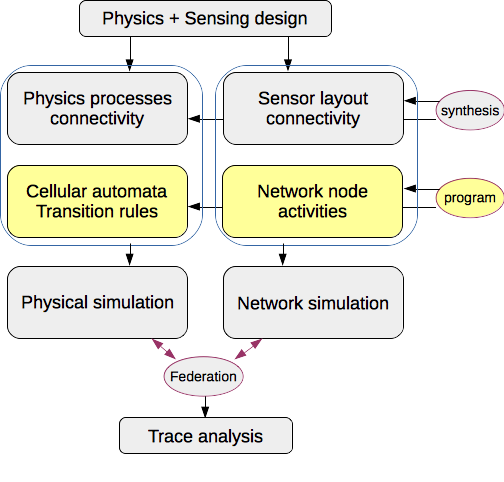
\includegraphics[width=6cm]{physics+sensorsFlow.png}
\caption{General flow for simulation with the physical simulation and the network simulation.
Both share coordination  informations such as geographical or geometrical points, clocking system,
and they can be coordinated during the simulation.}
\label{fig:physics+sensorsFlow}
\end{center}
\end{figure}


The interest of image anlysis is to  produce sets of  regions that share similar characteristics.
Analysis follows a conventional flow, starting from a picture comin from
photographies, maps, radar images, to obtain regions of interests, on which physical simulation  will
take place.

\begin{figure}[hbtp]
\begin{center} 
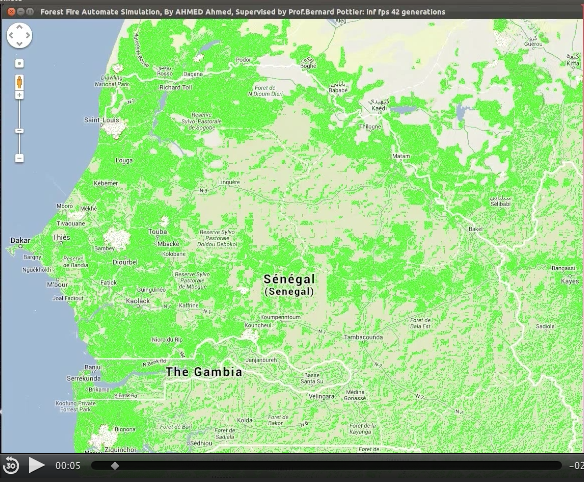
\includegraphics[width=10cm]{AhmedFire.png}
\caption{Example of a fire simulation  using Cellular Automata that have  states such as:
vegetation, burning, ashes.}
\label{fig:AhmedFire}
\end{center}
\end{figure}

A reference for processing on such regions are cellular automata
reproducing fire expansions of phenomenon consuming  vegetation.
Figure \ref{fig:AhmedFire} is extracted from a
movie demonstration where "fires" are started randomly to "eat" such vegetation report \cite{AhmedFire}. This
preliminary work was achieved on an Nvidia GPU.

The chapter will provide details on the production of   systems representing the physical
process working in harmony with the sensing systems.

\section{Image processing  flow for cellular system synthesis}

Thus,   modeling  physical regions automatically, or semi-automatically, following physical process 
characteristics, is certainly critical to lead both physical and control network  simulations jointly,
and synchronously. One can think of this as a sampling technique of the physical process sharing
a clock with the sensing network. Cellular automata are one way to implement the real world simulation,
starting from initial states and regions.


A general flow to obtain such regions  is  shown figure \ref{fig:pickcellFlow}~:
\begin{enumerate}
\item  preprocessing  images 
\item segmenting images into blocks
\item recognition of similar cells and grouping into regions
\item processing regions an obtaining skeleton images
\end{enumerate}

\begin{figure}[hbtp]
\begin{center} 
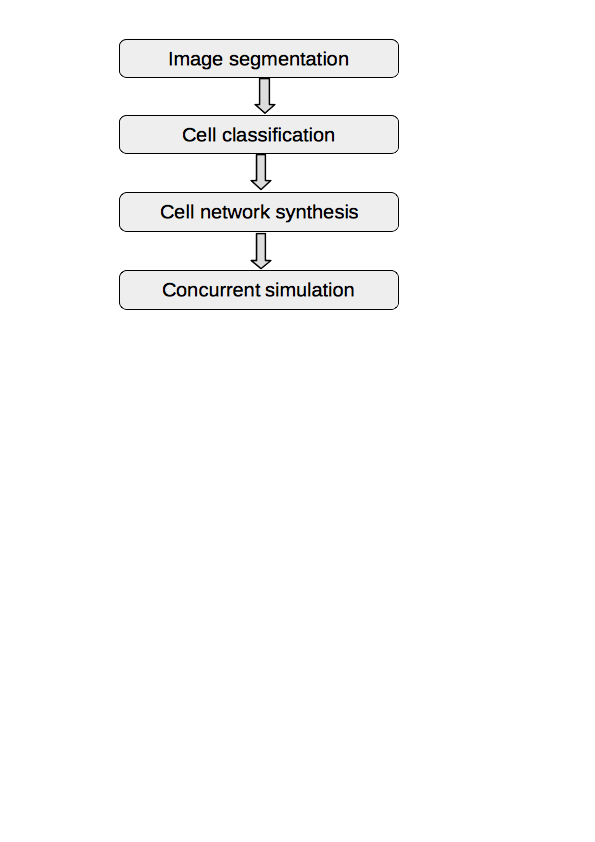
\includegraphics[width=6cm]{pickcellFlow.png}
\caption{Preparing cellular automata from image analysis: synthesis flow.}
\label{fig:pickcellFlow}
\end{center}
\end{figure}

Following this flow, higher level objects can be obtained, still with geographical definition in the case of
maps, or satellite imagery.

\subsection {Preprocessing for image preparation }

In the case of maps, geographic information is yet presented in a comprehensive way. However analyzing maps is still useful
to obtain information without the direct contact of an initial information system (GIS).
More difficult is the case of satellite or air  images, because the synthesis of objects necessitate
pre processing. Figure \ref{fig:sideBySide} shows an example of procesing achieved using common tools
for management of photographies. The initial view is a satellite image (left), while the right part displays an improved
view, with better contrasts.

\begin{figure}[hbtp]
\begin{center} 
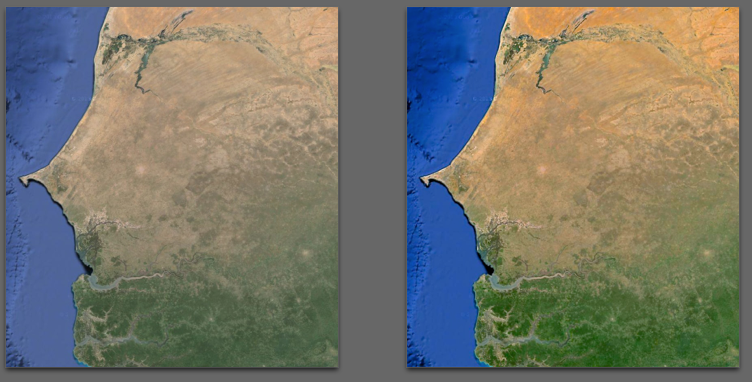
\includegraphics[width=10cm]{SenegalSideBySide.png}
\caption{Modifying original image for better contrasts or coulour selections. Image is a satellite view from Google Maps.}
\label{fig:sideBySide}
\end{center}
\end{figure}

These representations are coming from a very common image processing software 
allowing to change contrasts and colour mapping to fit tne necessity of the recognition.
Image processing paramers show the Red Green Blue statistic values in the original
and the modified image, with a better use of the value range in the second case
(Figure \ref{fig:colours1+2}).



\begin{figure}[hbtp]
\begin{center}
\leavevmode 
\begin{minipage}{6cm}
\begin{center} 
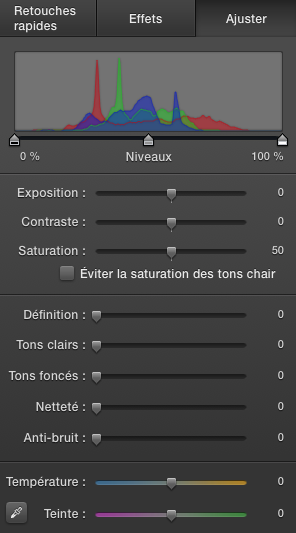
\includegraphics[width=6cm]{senegalColours.png} 
\end{center}
\end{minipage}~~~~~~~~~\begin{minipage}{6cm}
\begin{center} 
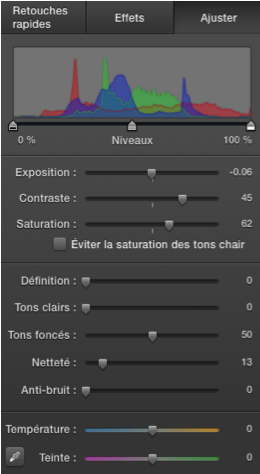
\includegraphics[width=6cm]{senegalColours2.png} 
\end{center}
\end{minipage}
\caption{RGB colour statistics for the left original picture, and its adaptation (right). The software
is Apple iPhoto, standard to any MacOs computer. Similar functions could be obtained from Linux GIMP,
and probably reimplemented from a Palette tool in NetGen.}
\label{fig:colours1+2}
\end{center}
\end{figure}
  
\subsection { Segmenting the image into cells}

To obtain regions, it is necessary to group zones of the image based on similarities of different kind.
The first operation is a fragmentation into blocks of different size and geometry. Of course,
squares, or rectangles are the simplest way to proceed, but other fragmentation techniques could also
be suitable and ease further stages in simulation. Cellular automata propose as example  an hexagonal
shape where each cell has 6 direct neighbours.

{\sc PickCell} has been implemented     to ease this fragmentation, in relation with 
further networks synthesis operations.

This tool reuse the {\sl Picking} framework presented Figure  \ref{fig:PickPoint1}. Beside the capability
to load images, and specify sensor positions, there is the ability to install a rectangular grid over the
image.


\begin{figure}[hbtp]
\begin{center} 
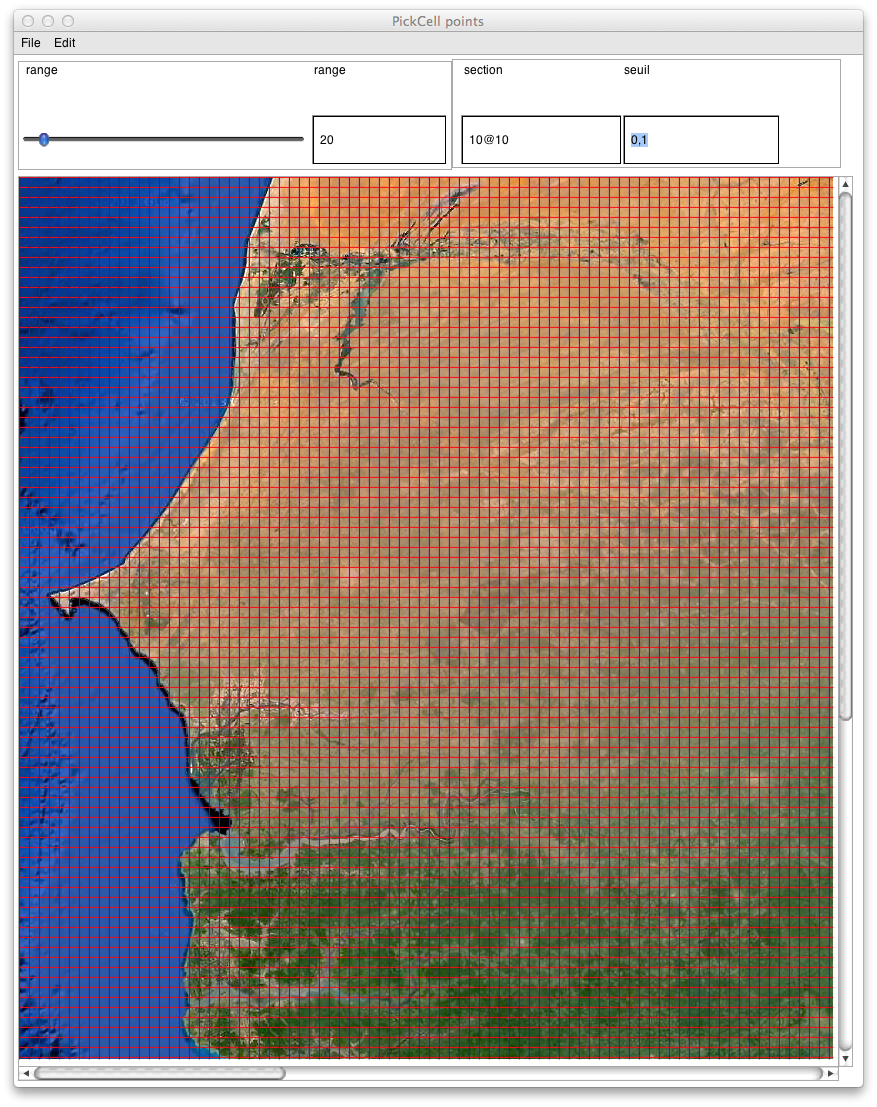
\includegraphics[width=10cm]{SenegalGrid10x10.png}
\caption{Using a 10@10 grid, the image is split into $10\times10$ pixels. 
Following the application, it is possible to specify $x  \times   y$ grids with $x  \neq  y$.}
\label{fig:SenegalGrid10x10}
\end{center}
\end{figure}

Having split the image into cells, it is now possible to classify thems around common properties.

\begin{figure}[hbtp]
\begin{center} 
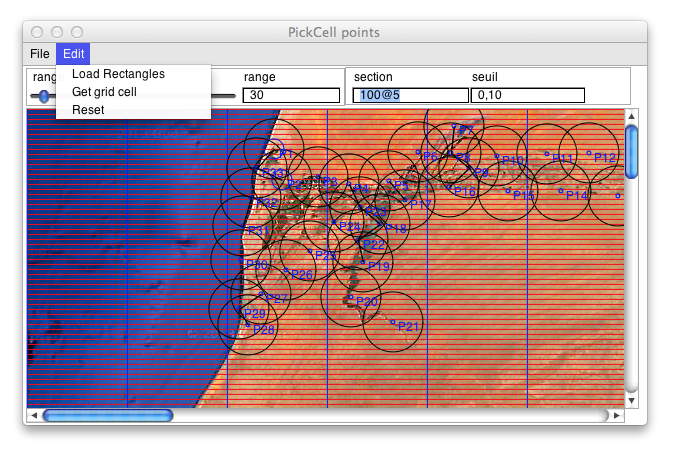
\includegraphics[width=10cm]{SenegalGetGridCell.png}
\caption{Rectangular grid, and sensor geometry specification. The Edit Menu {\sl Get Grid Cell} allows to go a step forward in the flow
to group cell togethers and form {\sl regions} of interest. Section \ref{sec:classification}}
\label{fig:SenegalGetGridCell}
\end{center}
\end{figure}

\subsection { Grouping cells  into classes}
\label{sec:classification} 
\subsubsection { Computing statistics}

From the menu shown Figure  \ref{fig:SenegalGetGridCell}, we obtain a new tool for region
specification and manipulation. As for the grid in segmentation, a new parameter allows to divide
the cell space according to pixel distributions.The choice of group distribution  can be more or less sophisticated.
To start by the begining, the following algorithm is applied to the whole cell grid, to obtain a set of $min, max, mean$ parameters
on each colour :

\begin{lstlisting}  
STEP 1
	for each cell in the grid
		for each pixel in the cell 
			 for each colour component in { R, G, B}
				 update (min(colour))
				 update (max(colour))
				 update (sum(colour))
		 for each colour component in { R, G, B}
			 update (mean(colour))
\end{lstlisting}

Following this step, we have $3 \times 3$ parameters set in each cell, thus allowing to compute
global image characteristics that will reflect the efficiency of the preprocessing:

\begin{lstlisting}  
STEP 2
	for each cell in the grid
		for each colour component in { R, G, B}
			update(minGlobal)
			update(maxGlobal)
			update(minMeanGlobal)
			update(maxMeanGlobal)
\end{lstlisting}


\begin{figure}[hbtp]
\begin{center} 
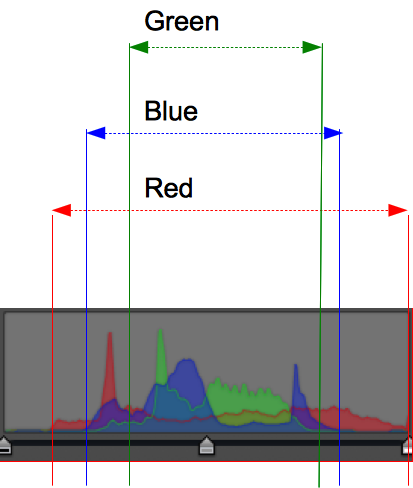
\includegraphics[width=6cm]{RGBDiagram.png}
\caption{From the preprocessing results shown Figure \ref,{fig:colours1+2},   we can guess min(colour), max(colour) for each
component in Red Green Blue.}
\label{fig:RGBDiagram}
\end{center}
\end{figure}

After this step and for each component in RGB space, we have global $[min,max] $ measures for:

\begin{itemize}
\item the value taken over the image (see Figure \ref{fig:RGBDiagram} )
\item the mean of values in each cell
\end{itemize}



\subsubsection { Grouping cell together }

We can use the values computed in each cell and globally to group cell togethers. For the minimum
and the maximum, and even the mean in each cell, a simple algorithm is as follows:

\begin{lstlisting}  
STEP3
	decide on a partition in N>1
	for each component in RGB
		discard any value out side the  [min,max]   interval found for the component
		produce N adjacent sub intervals   [min,max]  
\end{lstlisting}

In the case of $N=2$ the RGB min, max, or mean values in each cell will allow to {\sl classify}
each cell in an unique way in a $2^3$ interval space $(R_0,R_1) \times (G_0,G_1) \times (B_0,B_1) $.
The {\sl cube} of coordinates go from $0,0,0= 0$ to $1,1,1= 7$.
By selecting {\sl Get grid cell} shown Figure \ref{fig:SenegalGetGridCell} the classification tool appears.

What does this too is to allow the selection of $N$, then each cell is tne image is assigned to an interval
depending on its values. By selecting codes as defined above, the corresponding regions appear
an part of the original image. 


\begin{lstlisting}  
STEP4
	for each interval allocate a collection to record cells pertaining to this interval
	for each cell in the grid record the cell in its interval with the geographic position
\end{lstlisting}


\begin{figure}[hbtp]
\begin{center} 
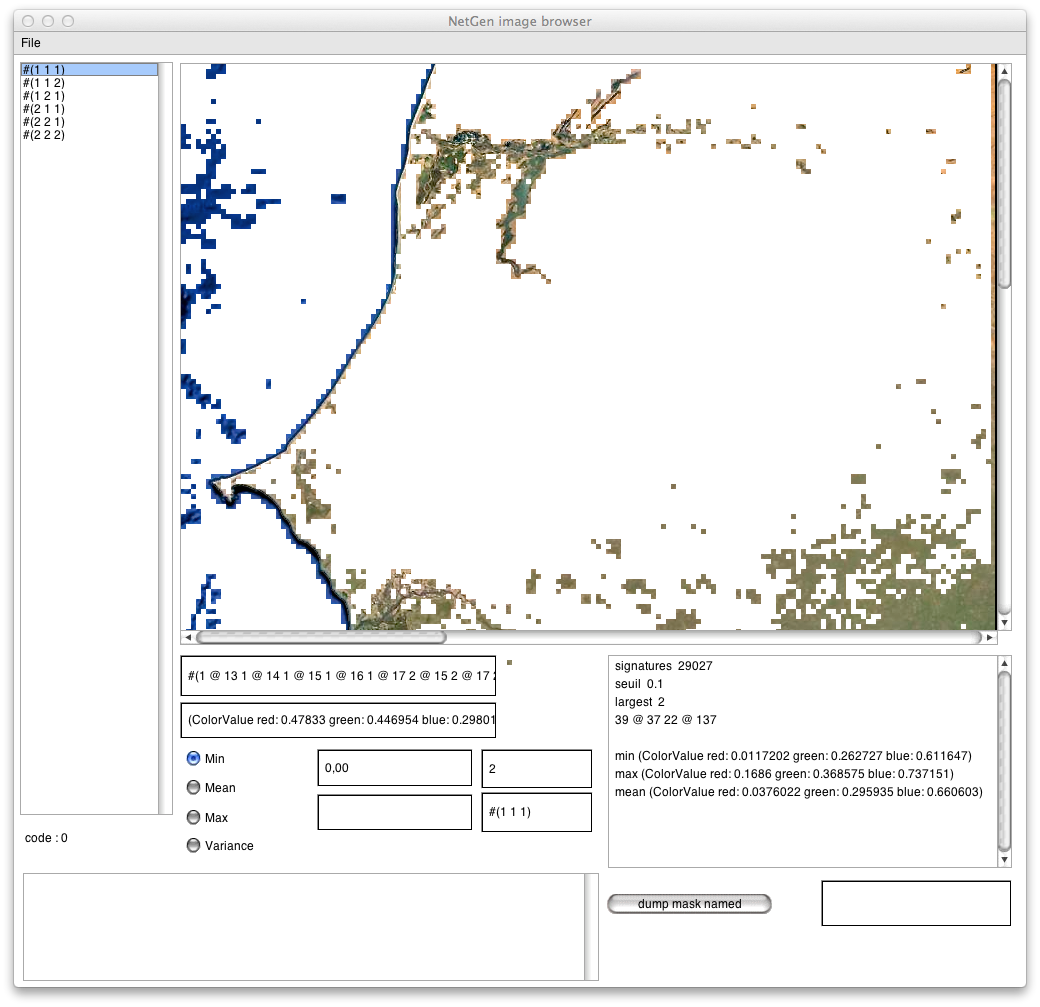
\includegraphics[width=12cm]{Senegal5x5code0.png}
\caption{Pixel class  browser displaying the region corresponding to code 0 : lowes interval in each component of R, G, B.
Shore and rivers appear as dark cell when the minimum criteria are selected. The partition is N=2, code is 0, for (R=1,G=1,B=1).}
\label{fig:Senegal5x5code0}
\end{center}
\end{figure}